% !TEX root=../../thesis.tex
\clearpage
\section{Case study of similiar systems}
\label{sect:backgroundExamples}
This section will present some similar systems and we will explain what the
systems tries to present.
\subsection{Zugmonitor}
\label{sub:subsection_zugmonitor}

In the Zugmonitor application (see \Ref{fig:zugmonitor}) each long-distance 
train in the German railway network has been plotted as a arrow on a German 
map. To illustrate the punctuality of each train, a colored circle has been 
added to each arrow if the train is delayed with varying color depending on 
how big the delay is. A time line is also displayed to see how the trains run 
on each step of the routes. 

\begin{figure}[!htbp]
	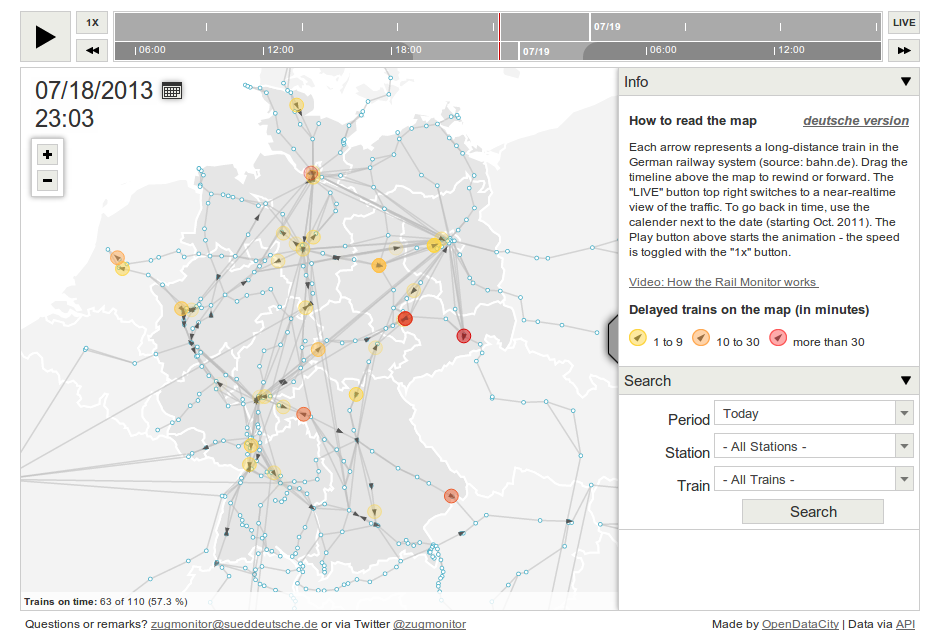
\includegraphics[width=0.7\textwidth,center]{zugmonitor.png}
	\caption[Zugmonitor]{Zugmonitor \cite{zugmonitor}}
	\label{fig:zugmonitor}
\end{figure}

\subsection{Vaguely live map of trains in the United Kingdom}
\label{sub:subsection_ukLiveMap}

The "Vaguely live map" system is a map which plots the relative location of 
each train in the United Kingdom (see \Ref{fig:ukLiveMap}). The plot fetches 
the departure time from the  National Rail website and calculates the relative 
location. The plot does not indicate whether the trains are on schedule or 
delayed, if one wants to check for delayes, one either has to do it manually 
on station, or for instance by checking a time table\cite{trainTimesUK}. Both 
the map and time table is developed on hobby basis by the same person. 

\begin{figure}[!htbp]
	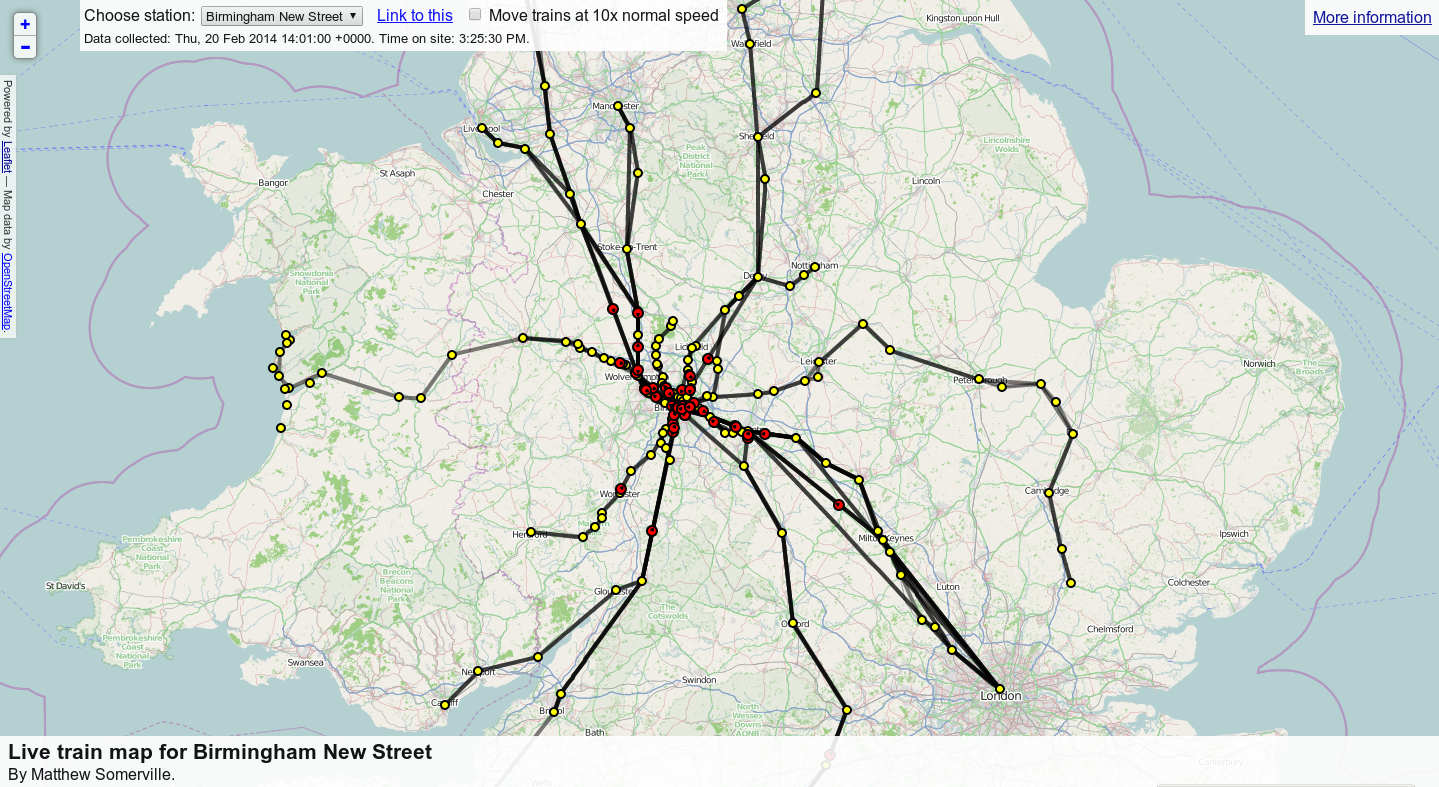
\includegraphics[width=0.7\textwidth,center]{live-train-map-for-Birminingham-new-street.png}
	\caption[UK live map]{UK live map \cite{ukLiveMap}}
	\label{fig:ukLiveMap}
\end{figure}

\subsection{MUNI Light Rail}
\label{sub:subsection_muniLightRail}

The "Muni light rail" system is a train graph based on the N-Judah line on the 
Muni Metro light railway line in San Francisco (see \Ref{fig:muniLightRail}). 
The train graph plots the schedule of the each train and the actual time each 
train uses. The chart auto updates every 10 seconds, and combined with being 
able to spot the difference between the schedule and the actual time, makes it 
easy to spot the delay of each train. As with \Ref{sub:subsection_ukLiveMap}
the "Muni light rail" system has been developed on a hobby basis.

\begin{figure}[!htbp]
	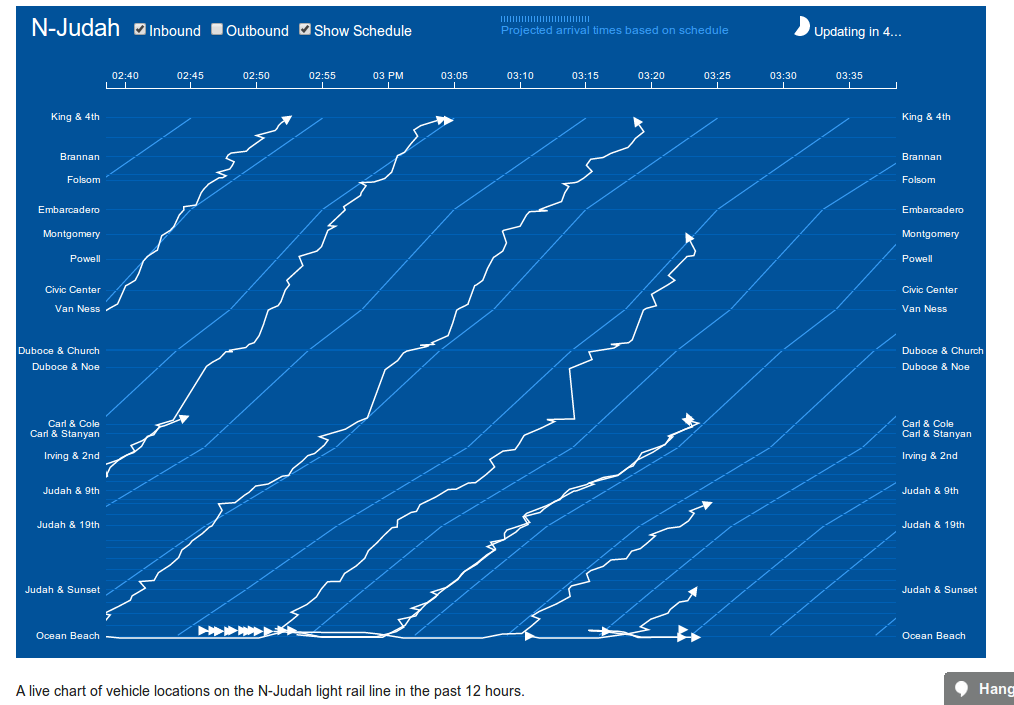
\includegraphics[width=0.7\textwidth,center]{visualizing-transit-delays.png}
	\caption[MUNI Light Rail]{MUNI Light Rail \cite{muniLightRail}}
	\label{fig:muniLightRail}
\end{figure}

\subsection{MiseryMap}
\label{sub:subsection_zugmonitor}

The MiseryMap (see \Ref{fig:miserymap}) shows how much different airports and 
the routes between them are delayed. The system also have a playback function 
to see the delays throughout the day. Since the plot sometimes also shows the 
weather conditions, the system gives the user the possibility to spot if the 
delays can be blamed on uncontrollable conditions. 

\begin{figure}[!htbp]
	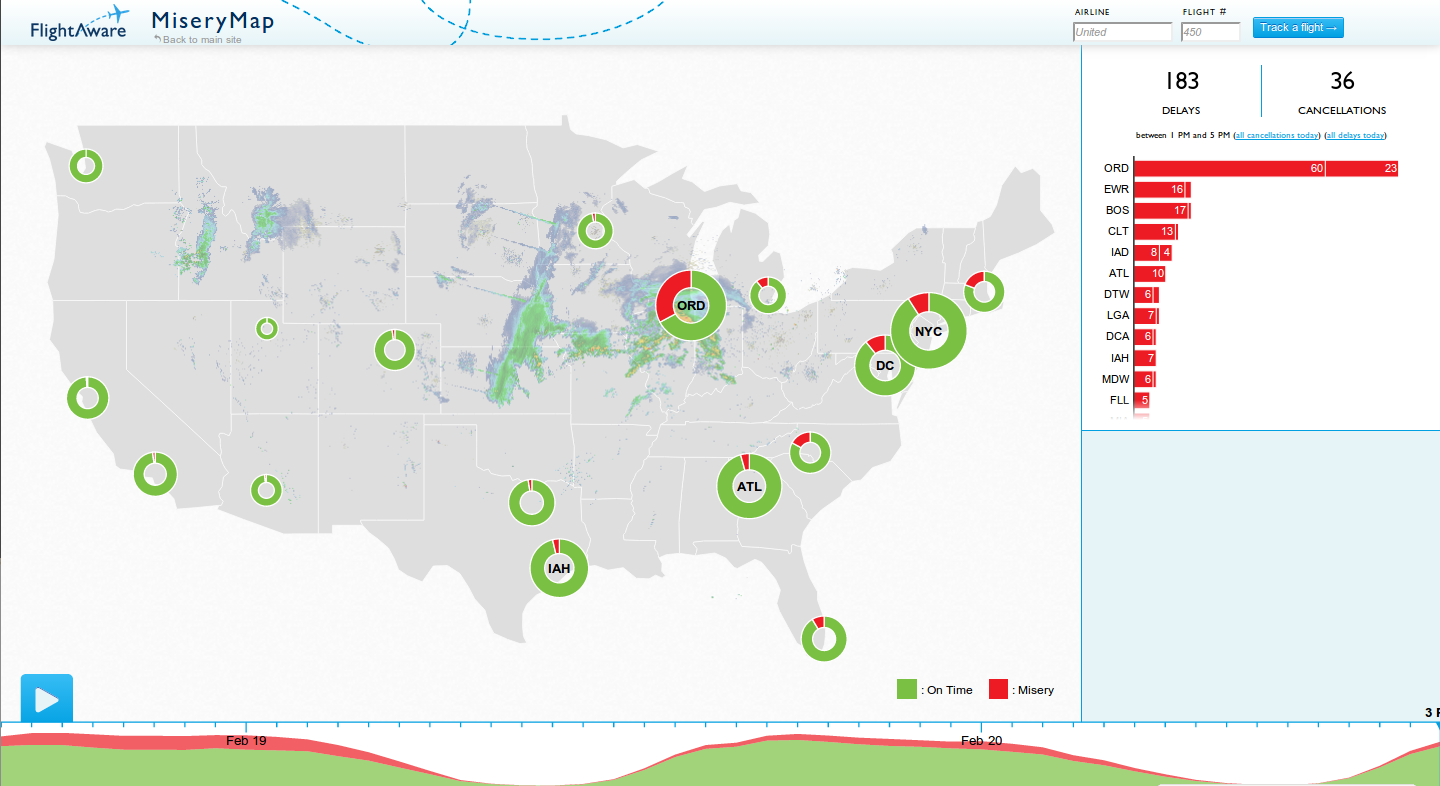
\includegraphics[width=0.8\textwidth,center]{MiseryMap.png}
	\caption[MiseryMap]{MiseryMap \cite{flightAware:MiseryMap}}
	\label{fig:miserymap}
\end{figure}
 
\subsection{Norwegian National Rail Administration}
\label{sub:subsection_jernbaneverket}

Jernbaneverket is the Norwegian governments agency for railway services 
\cite{jernbaneverketAbout}. As described in \Ref{sec:railway_operations}, 
Jernbaneverket is responsible for the infrastructure of all the railway 
network in Norway. Since they have responsibility for the infrastructure, 
they also collect data from points that each train passes, as described in 
\Ref{sec:back_data_sets}. Based on the collection of data, they have recently 
released a map (see \Ref{fig:jernbaneverket-punklighet}) over the punctuality 
on each track segment. The released map is a interactive map which shows a 
pop-up box containing the punctuality of the train segment clicked on, and the 
pop-up also shows which train routes that operates the train segment clicked 
on. The map, does not however, show more information if the user zooms inn, 
which is possible within the map itself, and has a static view of Norway and 
the railway. The map only shows the punctuality for passenger trains, and not 
freight trains and/or both.\\ 

To analyze each stretch, on a detailed level between each station,
Jernbaneverket has a internal system called TIOS.
TIOS can create a train graph which plots all trains that passes between all 
stations, \Ref{fig:jernbaneverket-tios} presents an example of the train graph 
between Oslo S and Drammen, where the red lines means planned time, black 
lines is actual time and the red circle indicates a a code for the cause of 
the delay. 

\begin{figure}[!htbp]
	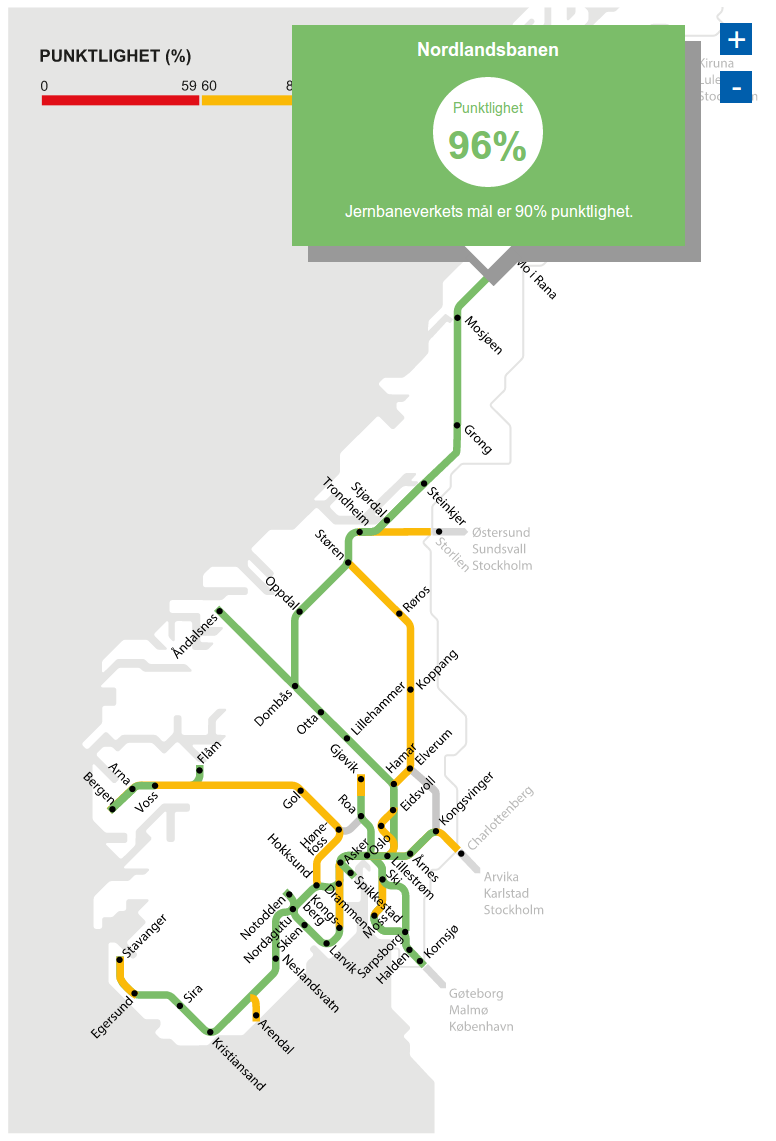
\includegraphics[height=0.4\textheight]{jernbaneverket-punklighet.png}
	\caption[JBV Punctuality map]{JBV Punctuality map \cite{jernbaneverketPunklighetKart}}
	\label{fig:jernbaneverket-punklighet}
\end{figure}
\begin{figure}[!htbp]
	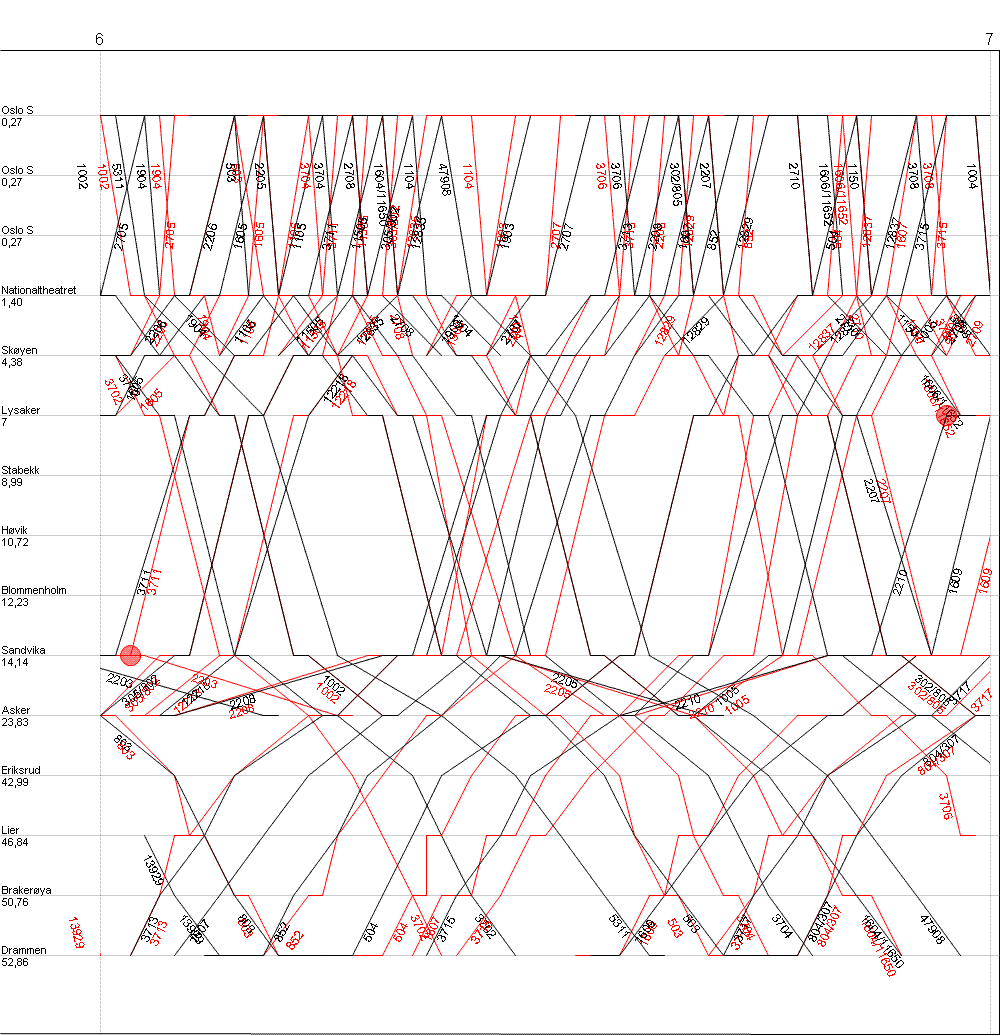
\includegraphics[width=\textwidth]{tios.png}
	\caption[TIOS]{TIOS\cite{jernbaneverketAbout}}
	\label{fig:jernbaneverket-tios}
\end{figure}

\subsection{Tåg.info}
\label{sub:subsection_taag.info}

Tåg.info\cite{taagInfo} is a Swedish system that tracks SJ\cite{svenskaJernban}
trains. The service gathers and processes data from Trafikverket\cite{trafikverket}. As with Cargonet (\Ref{sub:subsection_cargonet}),
Tåg.info provides a method (\Ref{fig:taag-info-kart}) of tracking live trains and visually see whether the trains are on schedule or delayed. 

Tåg.info also provides a method of analyzing national delays by presenting
graphs, \Ref{fig:taag-info-historik}. The service presents both a bar-chart
which presents the minutes of delays and the accumulated delays per day, and a
pie chart of the current status.

\begin{figure}[!htbp]
	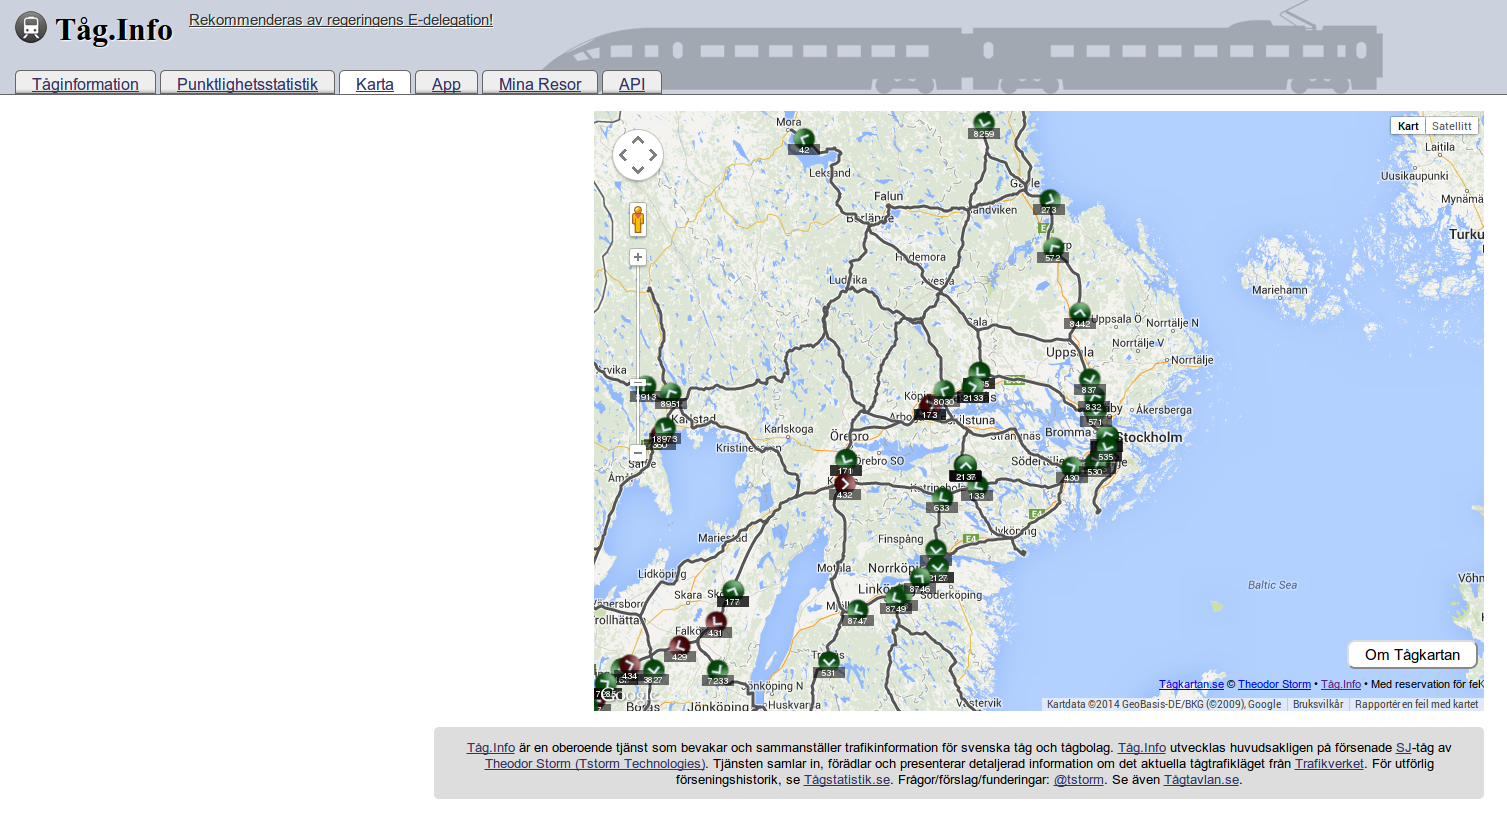
\includegraphics[width=0.7\textwidth,center]{taag-info-kart.png}
	\caption[Tåg.info map]{Tåg.info map
	\cite{taagInfo}}
	\label{fig:taag-info-kart}
\end{figure}

\begin{figure}[!htbp]
	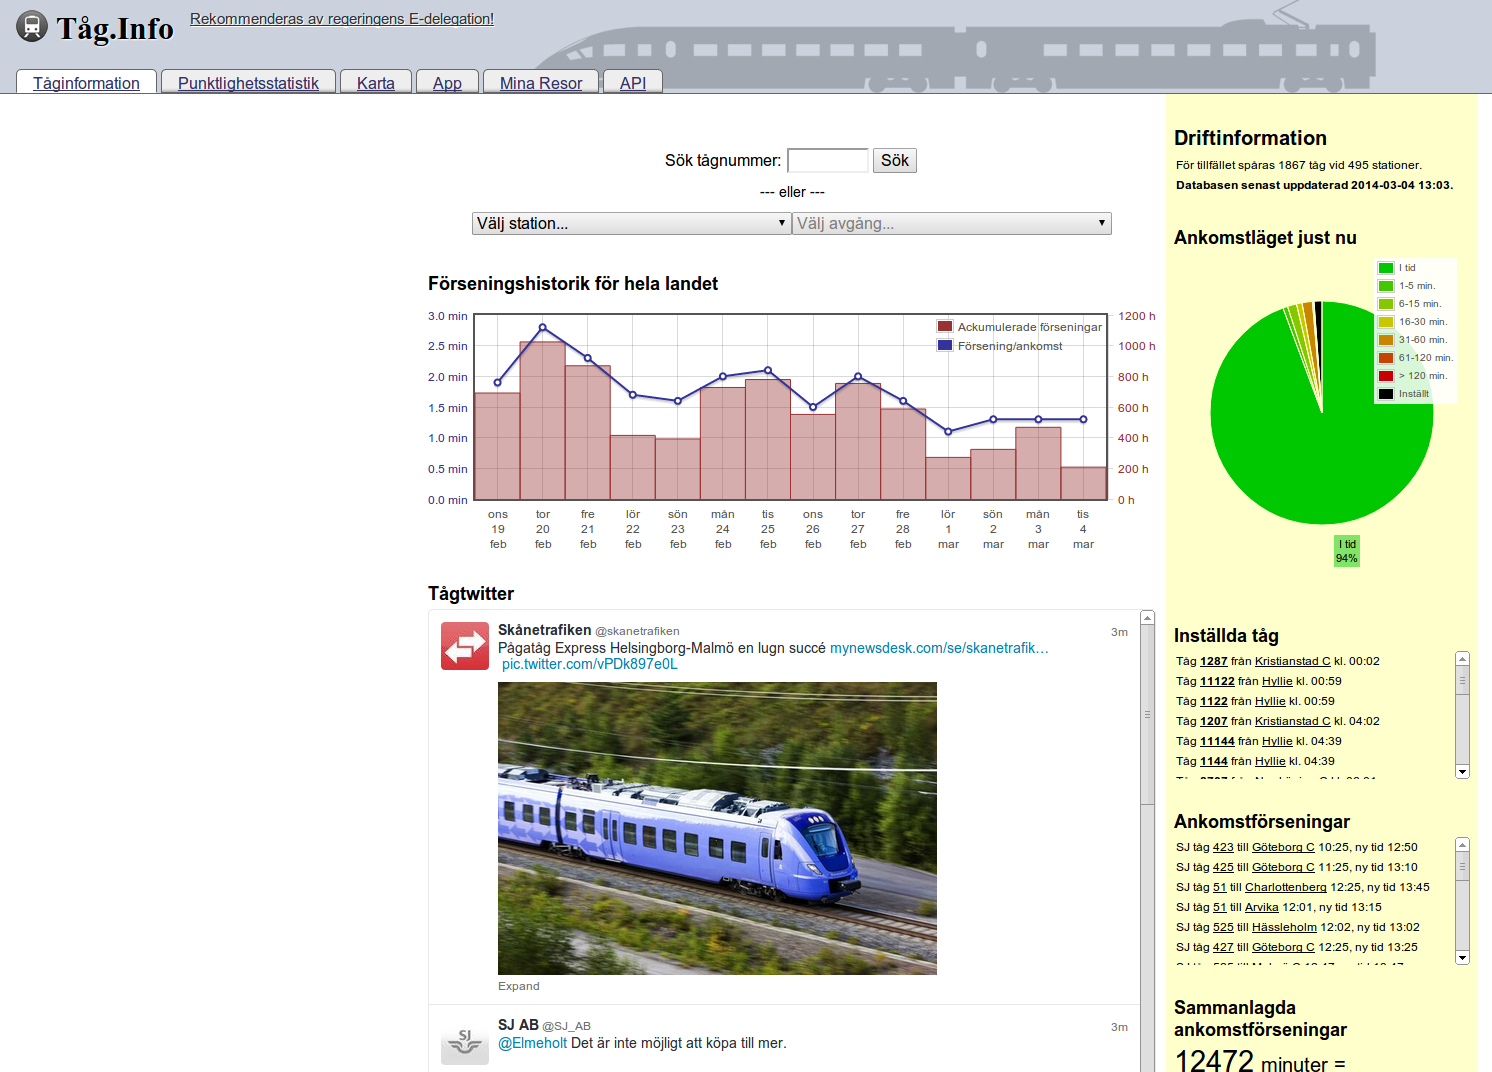
\includegraphics[width=0.7\textwidth,center]{taag-info-historik.png}
	\caption[Tåg.info history]{Tåg.info history
	\cite{taagInfo}}
	\label{fig:taag-info-historik}
\end{figure}


\subsection{SINTEF Presis}
\label{sub:subsection_sintefPresis}

The PRESIS\cite{sintefPresis} project is a collaboration between SINTEF\cite{sintef},
Transportøkonomisk Institutt\cite{transportOkonomiskInstitutt},
NTNU\cite{ntnu}, Jernbaneverket(\Ref{sub:subsection_jernbaneverket}) 
and the train operators Cargonet (\Ref{sub:subsection_cargonet}), NSB\cite{nsbForside}, and Flytoget\cite{flytoget}. The aim is to systematically improve the precision 
level in the railway system by developing methods, tools, and processes. During
the PRESIS project several prototypes for analyzing train delays have been 
developed.

A interaction plot, see \Ref{fig:krysningsinteraksjon}, plots the interaction
between two selected trains at a selected station. The interaction plot makes 
it easy to see if a train is delayed, and how the delayed train might affect 
another train. Since the interaction plot only plots the interaction between 
two trains, the plot makes it difficult to follow a delay back through the 
railway network to find the source. Due to not being able to track the delay
backwards, the plot is useful for individual trains, but are difficult to use
if one wants to look at the entire railway network or a large portion of it. \\

Publicly and internally the status of a train may differ whether a train are 
delayed or not. Public statistical data only shows delays on the final 
destination of the train, however all stations along the route show whether 
the train are on schedule or not on information screens on each station. Since 
Jernbaneverket collects data from all signal points along the route (see 
\Ref{fig:jernbaneverket-trafikkdata}), Jernbaneverket are able to track and 
plot the delays the train may experience along the route and not only at the 
end station. The PRESIS project has developed a prototype for such a plot, see 
\Ref{fig:live-punklighet}. Here the circles represent a station and the lines 
between the station have different colors which represent the punctuality 
between the stations, and the data which the plot is based on are listed to 
the right. The PRESIS project have also made it possible to get a time used 
over distance plot (see \Ref{fig:plot-spc-for-strekning}), based on the 
selected data in the Punctuality for routes plot. 

A plot based on time over distance, \Ref{fig:plot-spc-for-strekning}, plots the
actual time used by all trains that have driven that stretch in the selected
time period along with the running average. When plotting based on time over 
distance, the plot enables the possibility to spot where and
when trains have experienced problems on the selected stretch. They also have a
prototype plot which plots time used on station (see \Ref{fig:plot-spc-for-stasjonsopphold})
and other prototypes which is similar, just focusing on other parts of the
process.  %Bidragsplot, ikke tatt med.


%\begin{figure}[!htbp]
%	\centering
%	\begin{subfigure}{0.3\textheight}
%		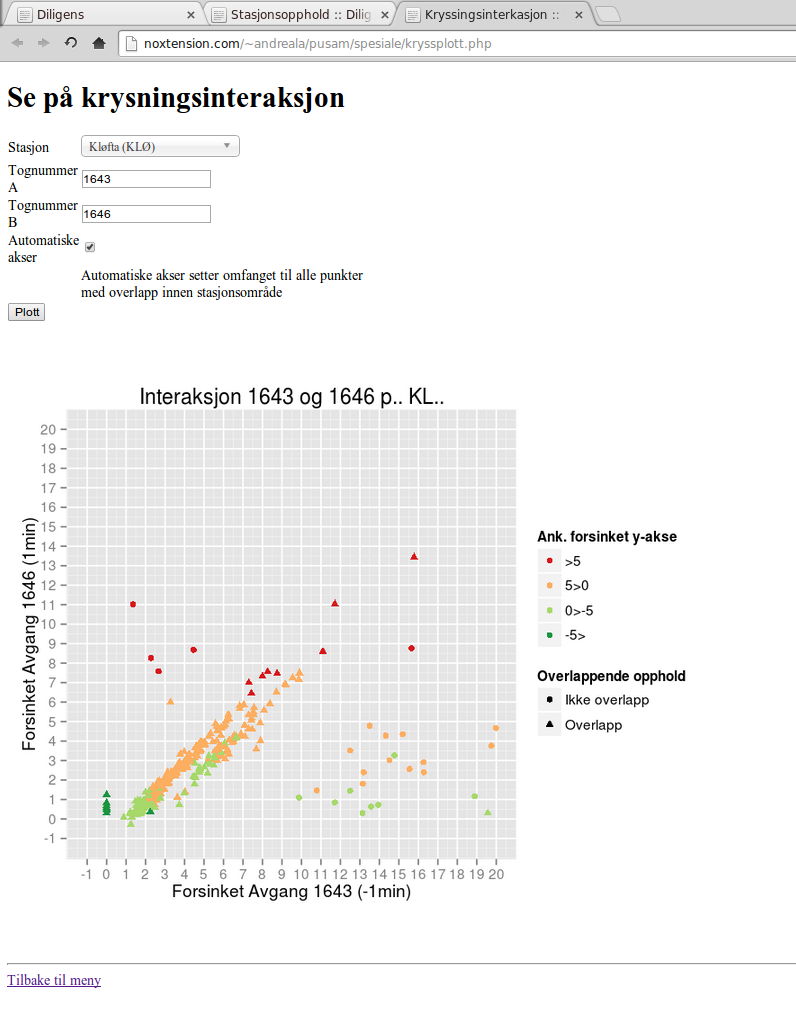
\includegraphics[width=0.3\textheight,center]{krysningsinteraksjon.png}
%		\caption[Train interaction plot]{Train interaction plot \cite{sintefPresis}}
%		\label{fig:krysningsinteraksjon}
%	\end{subfigure}
%	\begin{subfigure}{0.4\textheight}
%		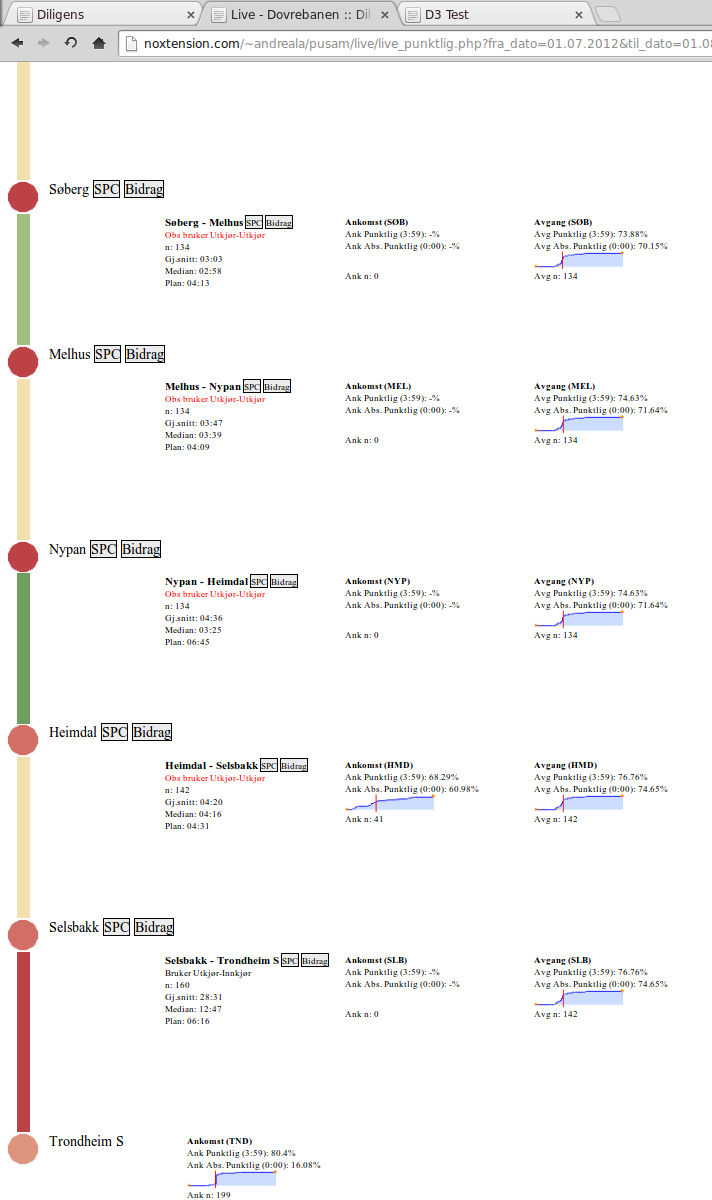
\includegraphics[height=0.4\textheight,center]{live-punklighet.png}
%		\caption[Route punctuality]{Route punctuality\cite{sintefPresis}}
%		\label{fig:live-punklighet}
%	\end{subfigure}
%	\caption[JBV Punctuality map and TIOS]{JBV Punctuality map and TIOS}
%	\label{fig:nbaneverket-punklighet_and_jernbaneverket-tios}
%\end{figure}

\begin{figure}[!htbp]
	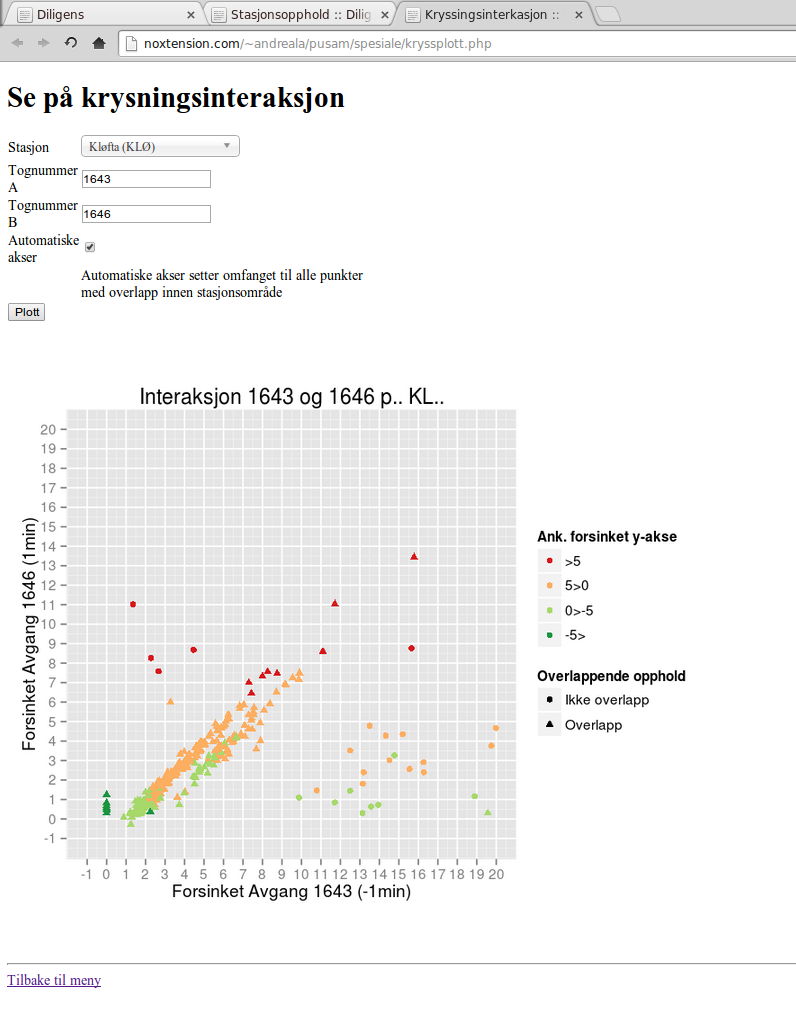
\includegraphics[width=\textwidth,center]{krysningsinteraksjon.png}
	\caption[Train interaction plot]{Train interaction plot \cite{sintefPresis}}
	\label{fig:krysningsinteraksjon}
\end{figure}

\begin{figure}[!htbp]
	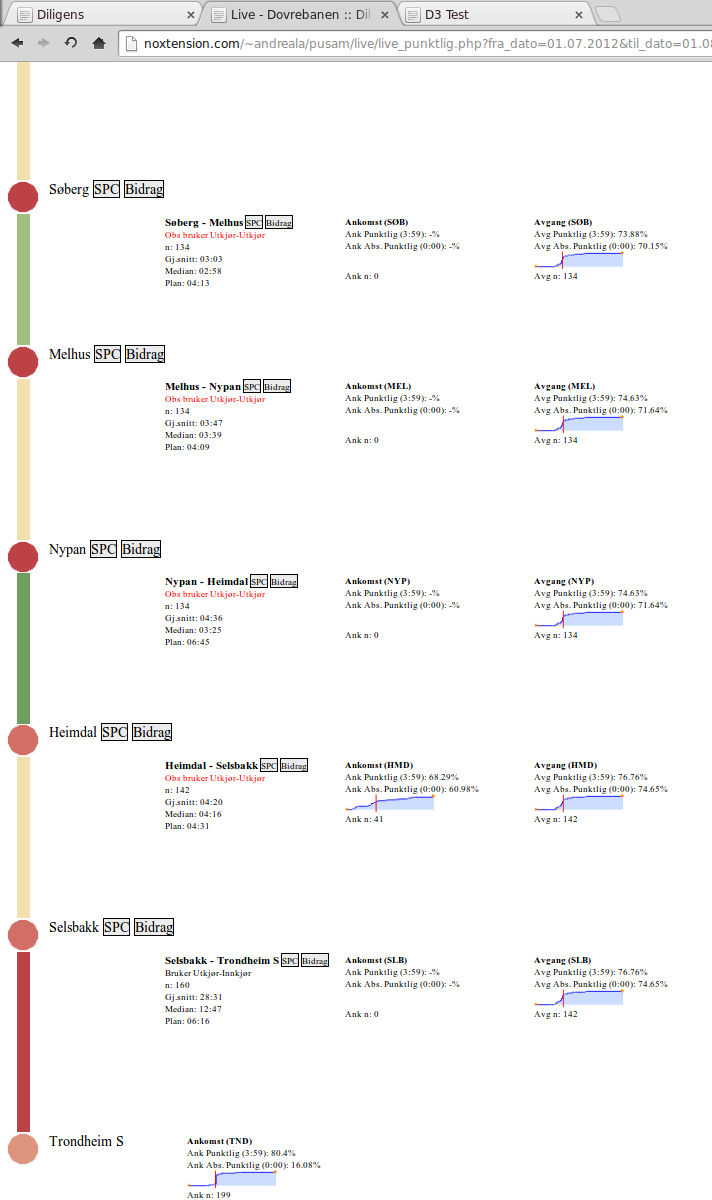
\includegraphics[height=\textheight,center]{live-punklighet.png}
	\caption[Route punctuality]{Route punctuality\cite{sintefPresis}}
	\label{fig:live-punklighet}
\end{figure}

\begin{figure}[!htbp]
	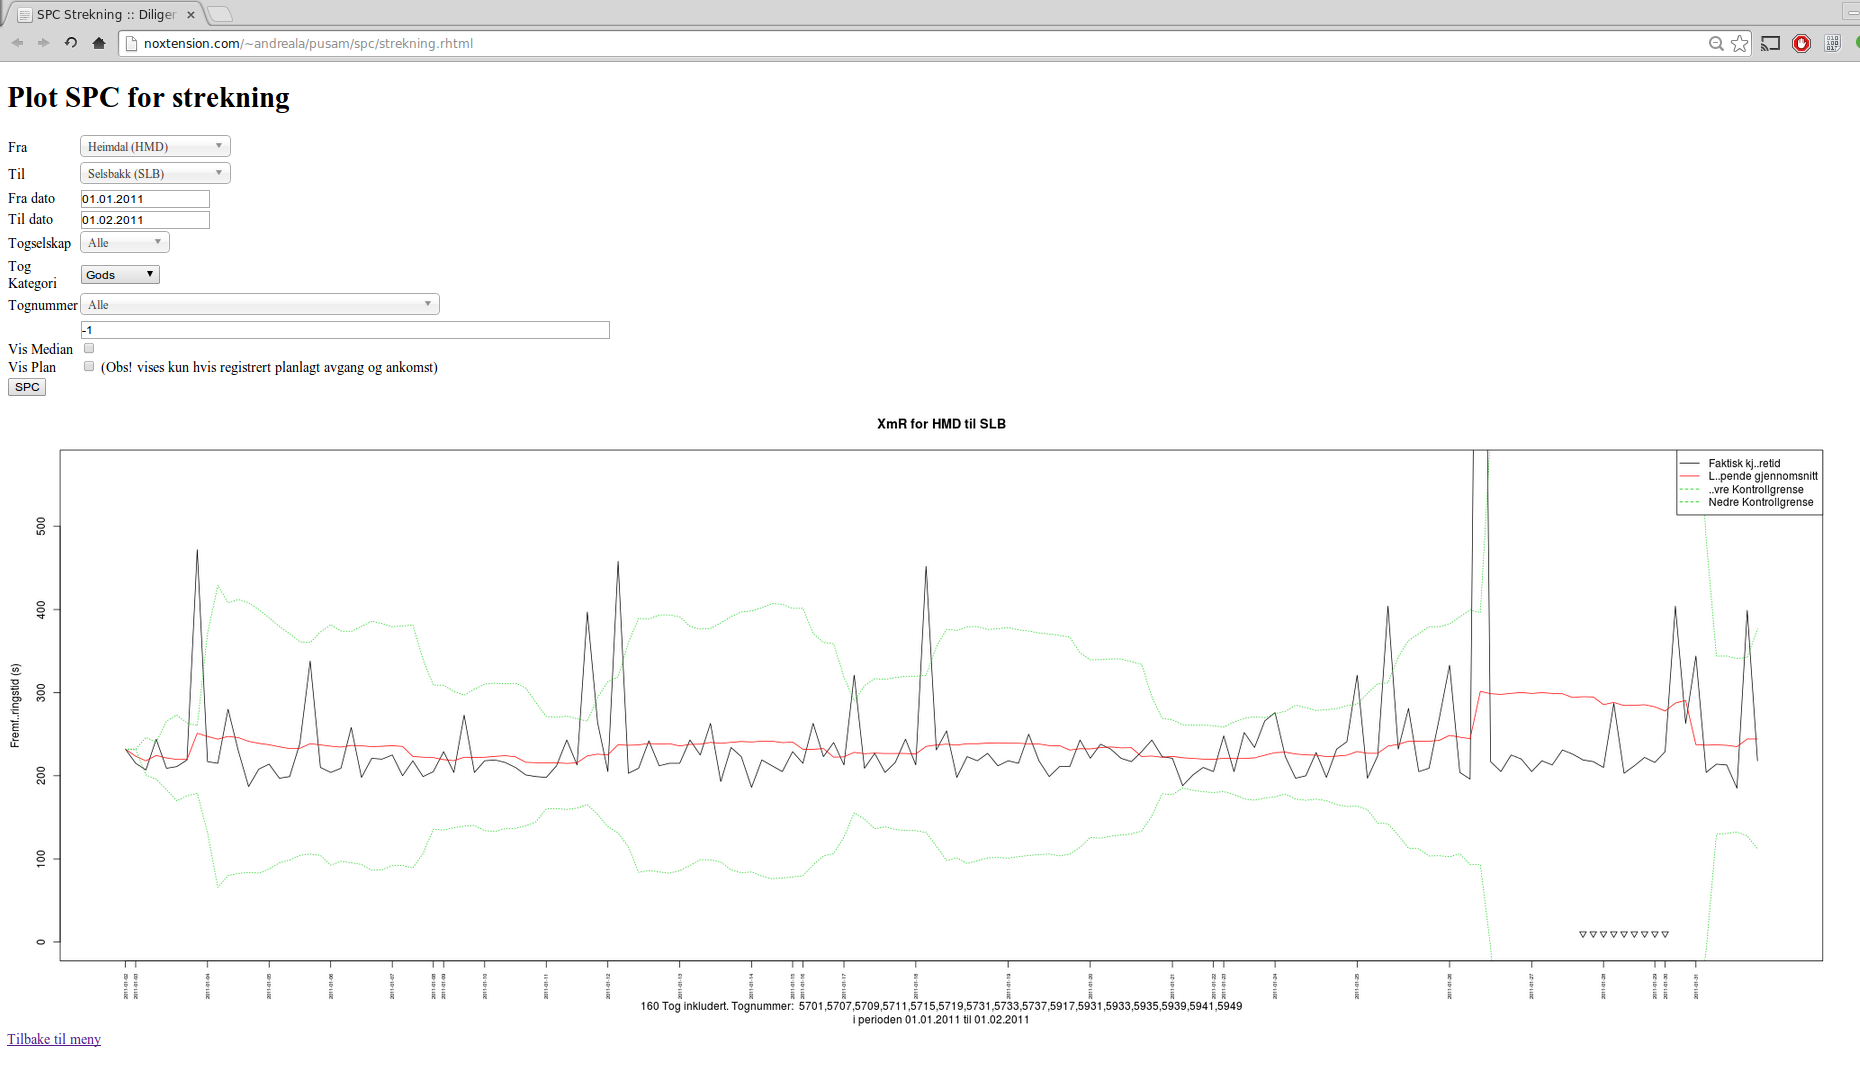
\includegraphics[width=\textwidth,center]{plot-spc-for-strekning.png}
	\caption[SPC Stretch]{SPC Stretch \cite{sintefPresis}}
	\label{fig:plot-spc-for-strekning}
\end{figure}

\begin{figure}[!htbp]
	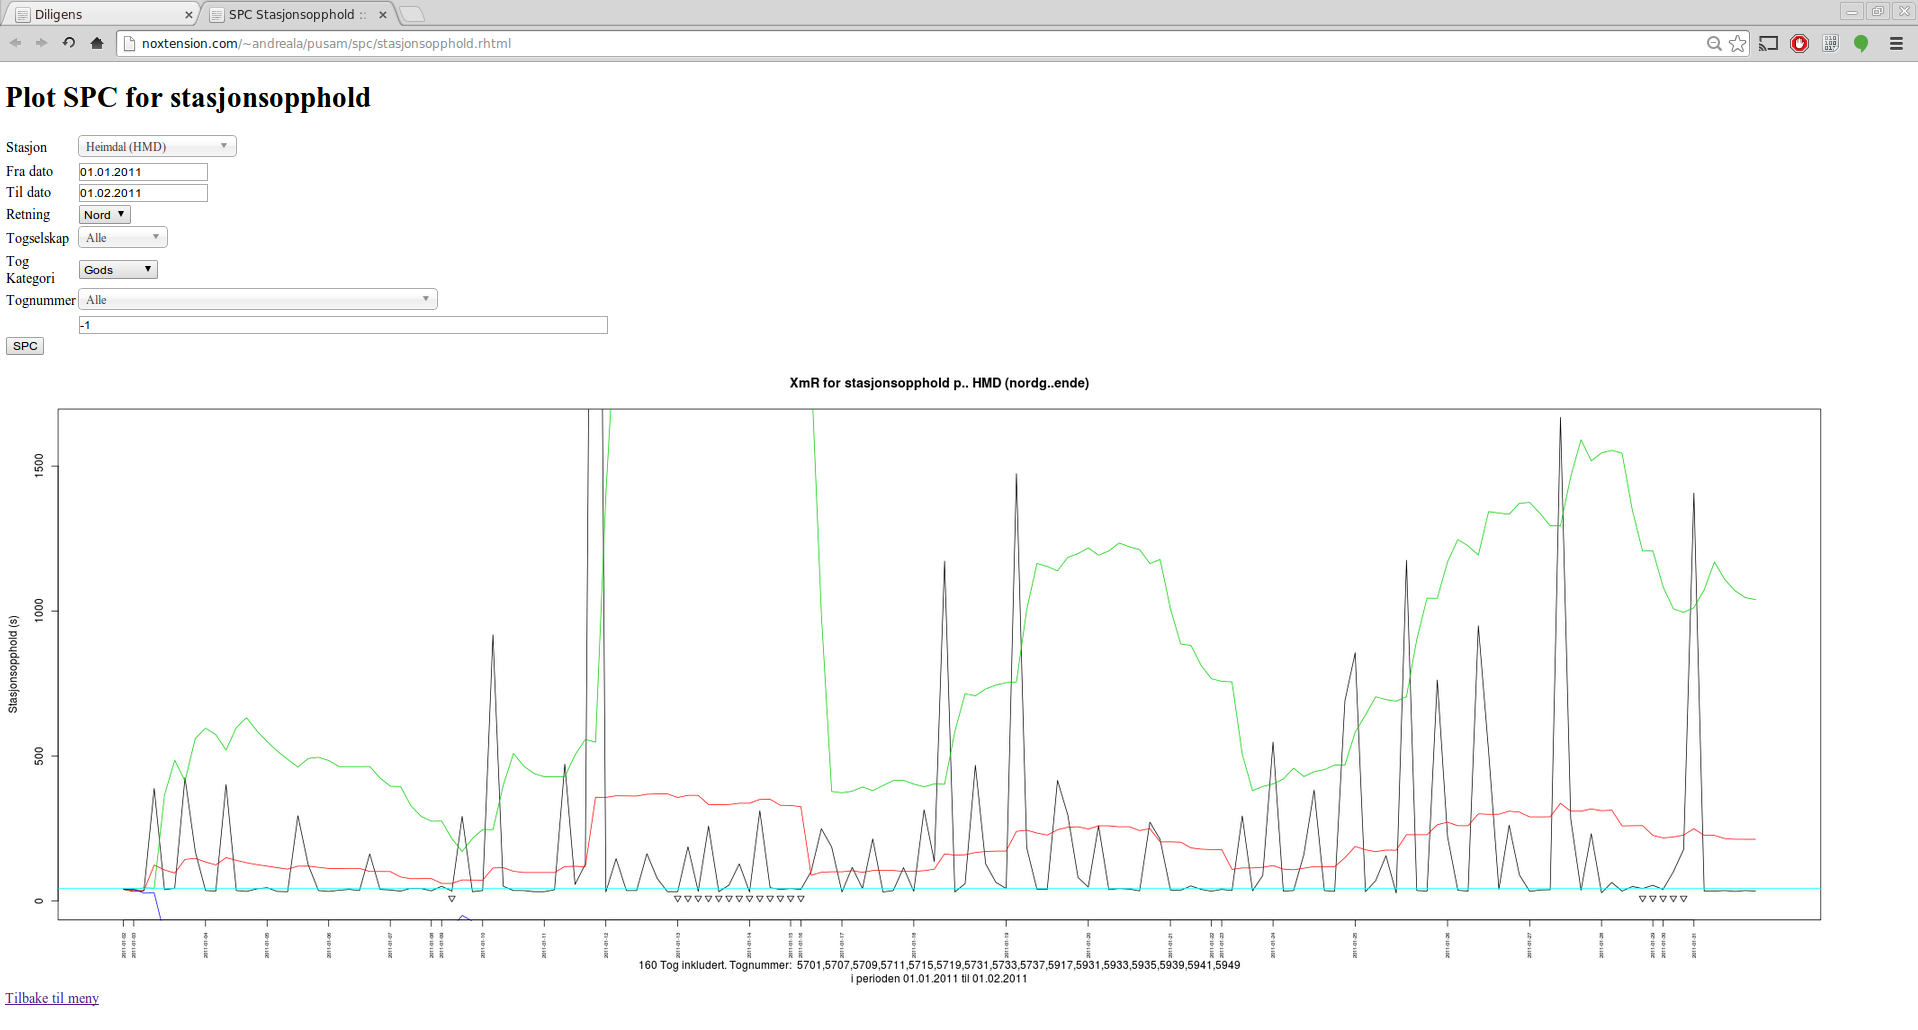
\includegraphics[width=\textwidth,center]{plot-spc-stasjonsopphold.png}
	\caption[SPC Station]{SPC Station \cite{sintefPresis}}
	\label{fig:plot-spc-for-stasjonsopphold}
\end{figure}

\begin{figure}[!htbp]
	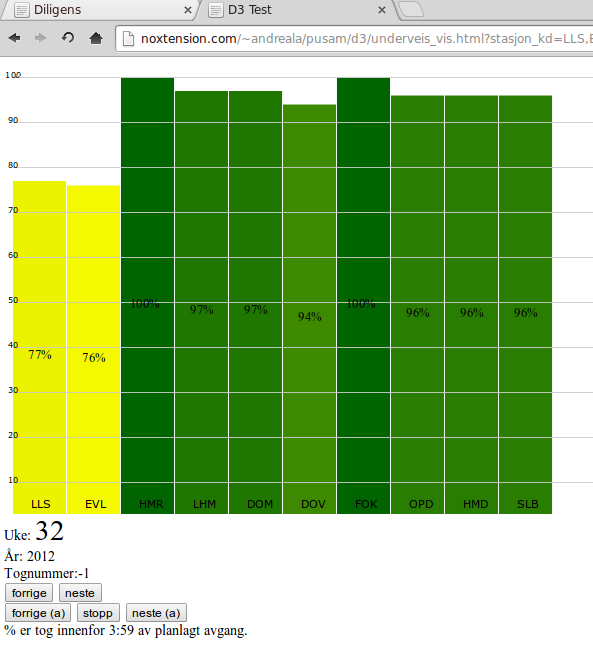
\includegraphics[width=\textwidth,center]{ukespunklighet.png}
	\caption[Weekly punctuality]{Weekly punctuality\cite{sintefPresis}}
	\label{fig:ukespunklighet}
\end{figure}

\subsection{Cargonet} % (fold)
\label{sub:subsection_cargonet}

% subsection subsection_sintefPresis (end)
Cargonet is a Norwegian company which provides intermodal transport on rails. 
To provide an effective tracking service for the customers, Cargonet provides 
an internal service for the users which tracks all trains belonging to Cargonet.
As can be seen in \Ref{fig:cargonet}, the system only shows a picture of the 
current status of each train. The system lacks the possibility to analyze 
every stretch individually and analyze trains and stretches over time.

\begin{figure}[!htbp]
	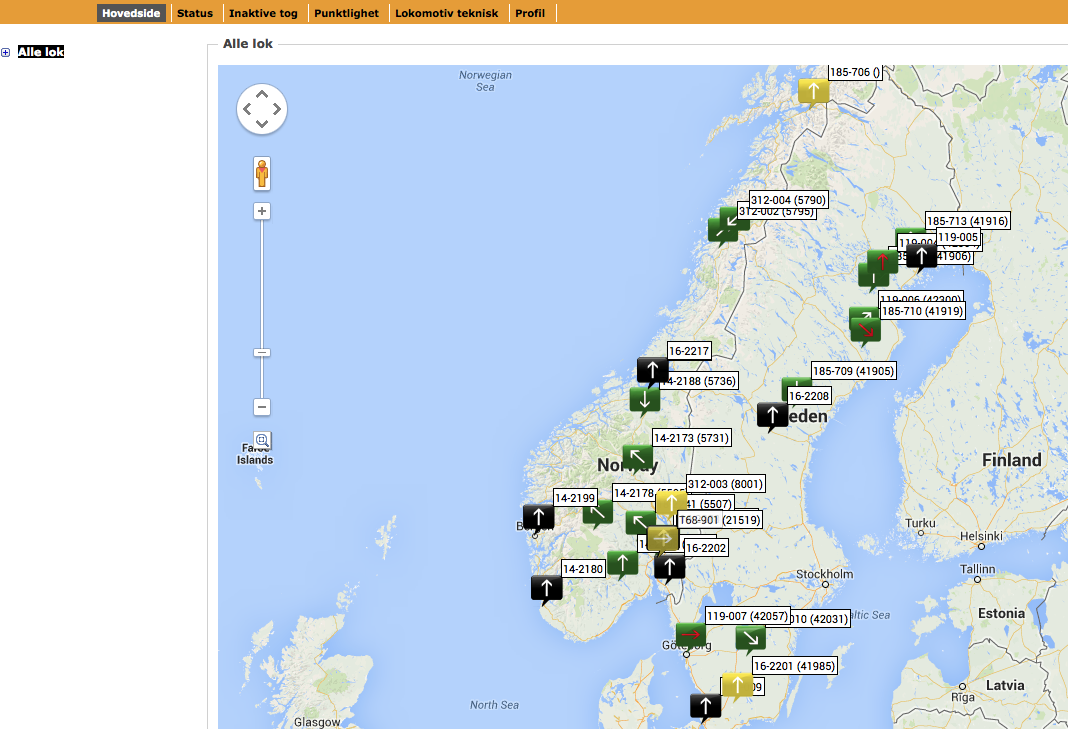
\includegraphics[width=\textwidth,center]{cargonet.png}
	\caption[Cargonet]{Cargonet \cite{cargonet}}
	\label{fig:cargonet}
\end{figure}

\begin{itemize}
	\item [] \textbf{How to read \Ref{fig:cargonet}}
	\item Red arrow:\hspace{4ex} Delayed.
	\item White arrow:\hspace{4ex} On time.
	\item Red box:\hspace{4ex} Locomotive driven 2km without carriages.
	\item Black box:\hspace{4ex} Locomotive without carriages.
	\item Yellow box:\hspace{4ex} Locomotive on time without schedule, or known position.
\end{itemize}

% subsection subsection_cargonet (end)
